% 1977 年山东B卷参考题 2：抛物线 y²=4x 与 x²=4y 所围曲边形（按源卷第 6 页布局）
% 坐标轴标 X、Y，两抛物线按源卷记号标 X²=4Y（上）与 Y²=4X（右下），交点 (0,0) 与 (4,4)
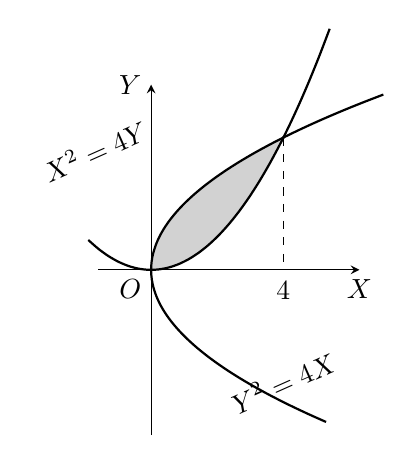
\begin{tikzpicture}[scale=0.42,>=stealth]
  % 坐标轴
  \draw[->] (-1.6,0)--(6.3,0) node[below] {$X$};
  \draw[->] (0,-5.0)--(0,5.6) node[left] {$Y$};
  \node[below left] at (0,0) {$O$};
  % 阴影区域：0≤x≤4 上 2√x 与 x²/4 之间
  \fill[gray!35]
    (0,0) plot[domain=0:4,smooth] (\x,{2*sqrt(\x)})
    -- plot[domain=4:0,smooth] (\x,{\x*\x/4}) -- cycle;
  % 抛物线 y²=4x（右开口，含左下延伸段）
  \draw[thick,domain=-4.6:5.3,smooth,samples=40] plot ({\x*\x/4},{\x});
  % 抛物线 x²=4y（上开口）
  \draw[thick,domain=-1.9:5.4,smooth] plot (\x,{\x*\x/4});
  % 交点 (4,4) 与虚线垂线
  \fill (4,4) circle (1.5pt);
  \draw[dashed] (4,4)--(4,0);
  \node[below] at (4,-0.05) {$4$};
  % 曲线标签（按源卷位置）
  \node[rotate=24] at (-1.7,3.6) {$X^2=4Y$};
  \node[rotate=24] at (4.0,-3.4) {$Y^2=4X$};
\end{tikzpicture}
